\section{Proposed Solution}
\label{sec:proposed_solution}

To address the limitations of the current centralized cloud computing model, we propose a novel decentralized cloud platform that combines the best aspects of traditional cloud services with the advantages of decentralized systems. Our solution is designed to tackle each of the key issues identified in the problem statement while introducing innovative features that enhance flexibility, security, and efficiency.

\subsection{Core Components of the Solution}

\subsubsection{Decentralized Infrastructure}
Our platform leverages a network of independent node providers, each capable of hosting and executing arbitrary workloads. This approach:
\begin{itemize}
    \item Mitigates vendor lock-in by offering a diverse ecosystem of providers
    \item Enhances resilience by distributing resources across nodes of different providers
    \item Improves resource utilization by tapping into underused computational capacity
\end{itemize}

\subsubsection{Reputation-Based Trust System}
\label{subsec:reputation_system}

Unlike typical Web3 solutions that rely on consensus mechanisms to mitigate the Byzantine Fault Tolerance (BFT) problem --- allowing up to 50\% (or a bit less on some platforms) of the network to be malicious --- our platform takes a different approach. We primarily rely on conventional legal contracts and Service Level Agreements (SLAs), supplemented by a robust blockchain-tracked reputation system. This dual approach ensures accountability through traditional means while providing an additional layer of trust and transparency.

In the anonymous blockchain space, an actor is more likely to behave maliciously than in the real world. In the real world there is a lot more at stake than in the blockchain space, an actor would be much less likely to behave maliciously, given that they risk suffering both legal and financial consequences for malicious behavior. Malicious behavior may still occur, but the potential benefit of such behavior needs to clearly compensate the potential cost, which may come in the form of a loss of the long-term financial benefit and the potential financial loss in the following legal processes, as analyzed in more details in Section~\ref{sec:math_model}.

Decent Cloud is designed with this in mind, and it focuses on incentivizing honest behavior and providing  high-quality service while implementing mechanisms to penalize poor performance or malicious actions. Good reputation is hard to earn, and it's easy to lose. Especially if big clients (with high reputation) are dissatisfied with the provided services.

\paragraph{Building Reputation:}
Node providers and developers accrue reputation through successful transactions and positive interactions on the platform:

\begin{itemize}
    \item Each completed transaction between a developer and a node provider results in a 2\% transaction fee, from which there is a 1\% increase in both parties' reputation scores.
    \item Consistent user satisfaction contributes to gradual reputation increases of node providers over extended periods and numerous transactions.
    \item Developers who rent many resources or spend significant amounts over longer periods of time will have higher reputation scores than those who do not.
\end{itemize}

\paragraph{Reputation Dynamics:}
Our system introduces an innovative approach to managing reputation:

\begin{itemize}
    \item Both node providers and developers build reputation through successful transactions.
    \item Rather than complicating the platform to autonomously track and judge honest behavior, we empower users to report and penalize malicious behavior.
    \item If dissatisfied with a service or collaboration, a user can choose to reduce another party's reputation. This action comes at a cost: the sender's reputation decreases by the amount spent, while the receiver's reputation decreases by a higher amount, such as 200%.
\end{itemize}

This mechanism offers several advantages:

\begin{itemize}
    \item Robustness: It's straightforward to implement and reason about.
    \item Quality Incentive: It motivates node providers to maintain high-quality service and prioritize user satisfaction.
    \item Resilience against Malicious Actors: Malicious node providers would quickly acquire poor reputations, limiting their ability to attract new users. Similarly, malicious developers quickly lose power to hurt the reputation of others, as they lose their own reputation in the process.
\end{itemize}

\paragraph{Reputation System Impact:}

This dynamic reputation system empowers users to make informed decisions when selecting node providers. It addresses trust and security concerns associated with decentralized systems while preserving the performance advantages of traditional cloud services. All reputation scores are publicly visible and immutably recorded on the blockchain, ensuring transparency and creating a reliable history of interactions and service quality.

\subsubsection{Efficient Resource Allocation}

Our platform can be used to ensure optimal resource allocation. For instance:
\begin{itemize}
    \item Task requirements can be matched with available node resources in real-time
    \item Dynamic load balancing optimizes resource utilization across the network
    \item Pricing is transparent and competitive, driven by market demand
\end{itemize}

This approach allows users to tackle the cost inefficiencies and opaque pricing models of traditional centralized providers.

\subsubsection{Enhanced Security and Privacy}

The system supports sensitive data processing and storage using Confidential Computing VMs, and also facilitates the rental of GPU nodes for Machine Learning (ML) and Artificial Intelligence (AI) training and inference applications at reasonable market prices, catering to different developer preferences. Some developers may opt for the lowest cost GPUs irrespective of node provider reputation and confidentiality guarantees, while others may prefer high-end GPUs with higher node provider reputation. This flexibility accommodates all developer categories, a feature unique to this platform.

For some use cases, such as storing and rotating tokens, certificates, and other secrets, developers will need nodes with additional security. For these use cases, platform will support Confidential Containers\cite{brasser2022trusted}.

To address data privacy and security concerns, our platform offers:
\begin{itemize}
    \item Support for Confidential Computing VMs, enabling secure processing of sensitive data
    \item End-to-end encryption for data in transit and at rest
    \item Granular control over data location and processing parameters
\end{itemize}

\subsection{Addressing Specific Challenges}

\subsubsection{Overcoming Vendor Lock-in}
Our platform's open architecture and standardized interfaces allow for easy migration between providers, addressing the vendor lock-in issue prevalent in centralized systems.

\subsubsection{Improving Control and Transparency}
Users have unprecedented visibility into the underlying infrastructure and can choose specific nodes or node providers based on their requirements, enhancing control and transparency.

\subsubsection{Enhancing Cost-Effectiveness}
The platform's market-driven pricing model and efficient resource allocation system ensure that users only pay for the resources they actually use, addressing the cost inefficiencies of traditional cloud services.

\subsection{Innovative Features}

\subsubsection{Wide Range of Applications}
Our platform supports diverse applications, from scientific high-performance computing and machine learning to web hosting and data storage, catering to a broad spectrum of user needs.

\subsubsection{DAO Governance}
We implement a Decentralized Autonomous Organization (DAO) model for platform governance, ensuring transparency and community-driven decision-making.

\subsubsection{Blockchain-Based Control Plane}
By running the control plane on a blockchain, we ensure transparent and immutable record-keeping for financial transactions and reputation tracking, while keeping the performance-sensitive data plane on the regular internet for optimal speed.

\subsection{Benefits for Stakeholders}

\subsubsection{For Developers}
\begin{itemize}
    \item Access to a diverse range of computational resources
    \item Flexibility to choose providers based on specific needs
    \item Potential for significant cost savings
\end{itemize}

\subsubsection{For Node Providers}
\begin{itemize}
    \item Opportunity to monetize unused computational resources
    \item Access to a global market of users
    \item Incentives for maintaining high-quality service through the reputation system
\end{itemize}

\begin{figure*}[h]
    \centering
    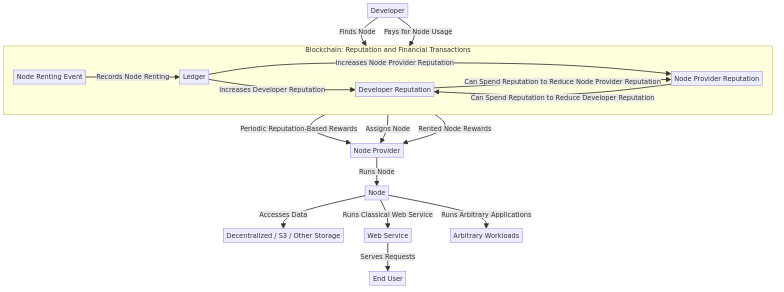
\includegraphics[width=\textwidth]{figures/proposed_architecture.png}
    \caption{Proposed platform architecture.}
    \label{fig:proposed-architecture}
\end{figure*}

Figure~\ref{fig:proposed-architecture} illustrates the architecture of our proposed platform, showcasing how these components interact to create a robust, efficient, and user-centric cloud computing ecosystem.

In the following sections, we will delve deeper into the technical details of each component, exploring how they work together to realize the full potential of decentralized cloud computing.
